\documentclass{article}
\usepackage{C:/Users/guitr/Documents/git_repositories/tpack/tpack}
% \usepackage{C:/Users/Admin-PC/Documents/git_repository/tpack/tpack}
% \usepackage{/home/tr0fin0/git_repositories/tpack/tpack}
% \usepackage{/home/Documents/git_repositories/tpack/tpack}
\usetikzlibrary{decorations.pathreplacing,calligraphy}

\title{OI201 - Systèmes d'Exploitation}
\project{Résumé Théorique}
\author{Guilherme Nunes Trofino}
\authorRA{2022-2024}


\makeatletter
\begin{document}\selectlanguage{french}
\maketitle

\newcommand{\comparison}[2]{
    \begin{remark}
        On considère les caractéristiques suivants:
        \begin{center}
            \begin{minipage}[t]{0.495\textwidth}
                \textbf{Avantages}:
                \begin{enumerate}[noitemsep]
                    #1
                \end{enumerate}
            \end{minipage}
            \begin{minipage}[t]{0.495\textwidth}
                \textbf{Inconvénients}:
                \begin{enumerate}[noitemsep]
                    #2
                \end{enumerate}
            \end{minipage}
        \end{center}
    \end{remark}
}


\newpage\tableofcontents

\section{Introduction}
\subfile{C:/Users/guitr/Documents/git_repositories/classes_ensta/intro.tex}
% \subfile{C:/Users/Admin-PC/Documents/git_repository/classes_ensta/intro.tex}
% \subfile{/home/tr0fin0/git_repositories/classes_ensta/intro.tex}
% \subfile{/home/Documents/git_repositories/classes_ensta/intro.tex}


\subsection{Information Matier}
\paragraph{Référence}Dans cette matière le but sera de comprendre comment une Système d'Exploitation marche.

\subsection{Histoire}
\begin{definition}\label{def:batchProcessing}
    Ordinateurs que n'exécutent qu'un seul programme à la fois font du \textbf{Batch Processing}.\\
    
    Dans ce cas le programme n'a pas besoin de partage les resources de l'ordinateur. Il pourrait acceder:
    \begin{enumerate}[noitemsep]
        \item toute la mémoire;
        \item tout le processeur;
        \item tous les périphériques;
    \end{enumerate}

    \begin{phrase}
        un système d'exploitation n'est utile que lorsqu'il y a plusieurs programmes
    \end{phrase}
\end{definition}

\section{Architecture}
\subsection{Architecture Matérielle}
\begin{definition}\label{def:architectureMaterielle}
    Décrit l'agencement interne de composants électroniques ainsi que leurs interactions.

    \begin{phrase}
        représente tous les ressources physiques disponibles et accessibles de l'ordinateur
    \end{phrase}
\end{definition}
\subsubsection{Architecture Von Neumann}
\begin{definition}\label{def:architectureVonNeumann}
    La même mémoire est utilisée pour stocker les instructions et les données des programmes.

    \begin{figure}[H]
        \centering\begin{tikzpicture}[]
            % modules
            \node[module] (CPU) {CPU};
            \node[module, right=of CPU] (MPU) {MPU};
            \node[module, right=of MPU] (BUS) {BUS};
            \node[module, above=of BUS] (MM0) {Mémoire Disque};
            \node[module, below=of BUS] (MM1) {Mémoire Vive};
            \node[module, right=of BUS] (PR0) {Périphériques};
            
            % connections
            \draw[<->] (BUS)--(PR0);
            \draw[<->] (CPU)--(MPU);
            \draw[<->] (MPU)--(BUS);
            \draw[<->] (BUS)--(MM0);
            \draw[<->] (BUS)--(MM1);
        \end{tikzpicture}
    \end{figure}
    On considère:
    \begin{enumerate}
        \item \textbf{CPU}: Control Process Unit;
        \item \textbf{MPU}: Memory Protect Unit;
        \item \textbf{BUS}: Connections entre les partis;
        \item \textbf{Mémoire}:
        \begin{enumerate}[noitemsep]
            \item \texttt{Mémoire Disque}: géré pour le Système de Fichiers:
            \begin{enumerate}[noitemsep]
                \item HD;
                \item SSD;
            \end{enumerate}
            \item \texttt{Mémoire Vive}: RAM;
        \end{enumerate}
        \item \textbf{Périphériques}:
        \begin{enumerate}[noitemsep]
            \item \texttt{Entrée / Sortie}, géré pour le Système de Fenêtres ou Shell:
            \begin{enumerate}[noitemsep]
                \item Clavier;
                \item Souris; 
            \end{enumerate}
            \item \texttt{Réseau}, géré pour la Pile de Réseau;
        \end{enumerate}
    \end{enumerate}

    \begin{remark}
        La Mémoire peut être interprété comme un Périphérique.
    \end{remark}
\end{definition}



\section{Software}


\subsection{Taille d'Information}
\subsubsection{bit}
\begin{definition}\label{def:bit}
    Valeur binaire, soit 0 ou soit 1. La plus petite unité d'information.
\end{definition}

\subsubsection{octet}
\begin{definition}\label{def:octet}
    Généralement, un ensemble de 8 bits binaires. La plus petite unité de mémoire adressable.
    
    \begin{remark}
        Nomme \textbf{byte} en anglais.
    \end{remark}
\end{definition}

\subsubsection{mot}
\begin{definition}\label{def:mot}
    Ensemble de plusieurs \texttt{octets}. La unité de mémoire manipulée naturellement par un processeur: 8, 16, 32, 64 ou 128 bits.

    \begin{remark}
        Nomme \textbf{word} en anglais.
    \end{remark}
\end{definition}

\subsubsection{Padding}
\begin{definition}\label{def:padding}
    Consiste à garantir que la taille des données soit compatible avec les algorithmes utilisés.
\end{definition}

\subsubsection{Endianness}
\begin{definition}\label{def:endianness}
    Convention pour lire les octets dans un mot:
    \begin{enumerate}[noitemsep]
        \item \textbf{big endian}: On commence par l'octet plus grand, gauche à droite;
        \item \textbf{little endian}: On commence par l'octet plus petit, droite à gauche;
    \end{enumerate}
    
    \begin{example}
        On considère le code suivante:
        \begin{scriptsize}\myRISCV
            \begin{lstlisting}
    variable = {0x11, 0x22, 0x33, 0x44};
    
    .word 0x11223344    # code little endian, plus commun
    
    .word 0x44332211    # code big endian
            \end{lstlisting}
        \end{scriptsize}
    \end{example}

    On peut convertir les variables d'une codage à une autre avec l'\href{https://codereview.stackexchange.com/questions/151049/endianness-conversion-in-c}{algorithme}.
\end{definition}


\subsection{Noyau}
\begin{definition}\label{def:noyau}
    Partie fondamentale du Système d'Exploitation, responsable privilégié pour gérer les ressources de l'ordinateur:
    \begin{enumerate}[noitemsep]
        \item \texttt{allocation}: comment répartir la mémoire
        \item \texttt{ordonnancement}: définir quel processus s'exécute à un instant;
    \end{enumerate}
    
    \begin{remark}
        Nomme \textbf{kernel} en anglais.
    \end{remark}
\end{definition}

\subsubsection{Service}
\begin{definition}\label{def:service}
    Programme qui organise le partage de ressources de l'ordinateur.
\end{definition}

\subsubsection{Pilote Périphérique}
\begin{definition}\label{def:pilotePeripherique}
    Service responsable pour organiser le partage des périphériques de l'ordinateur en communicant avec le \textbf{noyau} \ref{def:noyau}.
    
    \begin{remark}
        Nomme \textbf{driver} en anglais.
    \end{remark}
\end{definition}


\subsection{Ordonnanceur}
\begin{definition}\label{def:ordonnanceur}
    Composant du noyau du système d'exploitation choisissant l'ordre d'exécution des processus sur les processeurs d'un ordinateur, c'est à dire l'attribution de travaux à des resources, à partir d'une Politique d'Ordonnancement \ref{def:politiqueOrdonnancement} implémente.
    
    \begin{remark}
        En anglais, l'Ordonnanceur est appelé \textbf{scheduler}.
    \end{remark}
    L'allocation statique de mémoire n'est pas un ordonnancement.
\end{definition}

\subsubsection{Politique d'Ordonnancement}
\begin{definition}\label{def:politiqueOrdonnancement}
    Contraintes permettant de décider à tout instant quel travail exécuter par les travaux prêts en considérant les aspects suivants:
    \begin{enumerate}
        \item \textbf{Coût de Préemption}, coût pour interrompre un travail:
        \begin{enumerate}[noitemsep]
            \item \texttt{élevé}: ;
            \item \texttt{faible}: ;
        \end{enumerate}
        \item \textbf{Coût de Migration}, coût pour changer d'une ressource à une autre:
        \begin{enumerate}[noitemsep]
            \item \texttt{élevé}: ;
            \item \texttt{faible}: ;
        \end{enumerate}
        \item \textbf{Critère d'Optimisation}, peut varier d'application à application:
        \begin{enumerate}[noitemsep]
            \item \texttt{débit}: maximiser le nombre de tâches faites;
            \item \texttt{latence}: minimiser les temps de réponse à des évènements;
            \item \texttt{équité}: faire en sorte que toutes les t6aches aient accès aux ressources;
        \end{enumerate}
    \end{enumerate}
\end{definition}

\subsection{Algorithme d'Ordonnancement}
\begin{definition}\label{def:algorithmeOrdonnancement}
    Représente la Politique d'Ordonnancements désiré pour le noyau. On peut classifier de la façon suivante:
    \begin{enumerate}
        \item \textbf{Statique}: plan d'ordonnancement est décide avant l'exécution;
        \begin{enumerate}[noitemsep]
            \item McNaughton;
        \end{enumerate}
        \item \textbf{Dynamique}: plan d'ordonnancement est décide pendant l'exécution;
        \begin{enumerate}[noitemsep]
            \item \texttt{Non Préemptif}: les tâches ne peuvent pas être interrompre;
            \begin{enumerate}[noitemsep]
                \item FIFO;
            \end{enumerate}
            \item \texttt{Préemptif}: les tâches peuvent être interrompre;
            \begin{enumerate}
                \item Priorité Statique: priorité des travaux ne change pas;
                \begin{enumerate}[noitemsep]
                    \item RM;
                    \item Round-Robin;
                \end{enumerate}
                \item Priorité Dynamique: priorité des travaux peut changer;
                \begin{enumerate}[noitemsep]
                    \item EDF;
                    \item Multi-Level Feedback;
                \end{enumerate}
            \end{enumerate}
        \end{enumerate}

    \end{enumerate}
\end{definition}
    
\subsubsection{FIFO}
\begin{definition}
    Algorithme d'Ordonnancement a First in First Out; First Come First Served, FCFS; Premier Entré Premier Sorti, PEPS.

    \begin{example}
        Une imprimante est partagée entre 20 personnes. Dans quel ordre faire les impressions?
    \end{example}
    \comparison{
        \item optimal s'il y a une seule ressource;
        \item aucune connaissance sur les travaux;
    }{
        \item pas de prise en compte de priorités;
        \item pas de parallélisation du CPU;
    }
    \begin{remark}\label{def:queue}
        File d'Attente, en anglais \textbf{queue}, implémente FIFO.
    \end{remark}
\end{definition}

\subsubsection{LIFO}
\begin{definition}
    Algorithme d'Ordonnancement a Last in First Out, Dernier Entré Premier Sorti, DEPS
        \begin{example}\label{def:stack}
            Pile, en anglais \textbf{stack};
        \end{example}
\end{definition}

\subsubsection{SJF}
\begin{definition}
    Algorithme d'Ordonnancement a Shortest Job First
\end{definition}

\subsubsection{EDF}
\begin{definition}
    Algorithme d'Ordonnancement a Earliest Deadline First
\end{definition}

\subsubsection{McNaughton}
\begin{definition}
    Algorithme d'Ordonnancement a McNaughton
    \begin{example}
        4 étudiants veulent faire 60 abdominaux chacun, 1 par seconde, en y passant un minimum de temps. Il n'y a que 3 tapis. Comment le faire?
    \end{example}
    \begin{resolution}
        Il y a 240 secondes de travail à faire, 60 abdominaux chaque étudiant. Donc le temps minimum pour tout faire est de 80 secondes en considérant que les tapis sont utilisés au même temps. À la fin on aura:
        \begin{figure}[H]
            \centering
            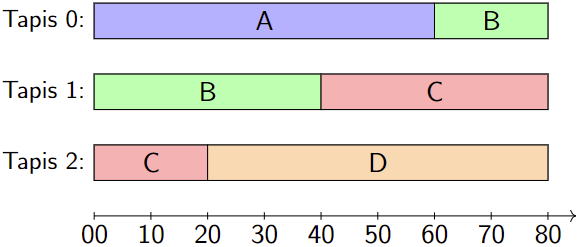
\includegraphics[width=60mm]{images/mcNaughton_output.png}
        \end{figure}
    \end{resolution}
    \comparison{
        \item optimal sur multi-processeur;
    }{
        \item faire des migrations;
        \item connaître tous les travaux;
    }
\end{definition}

\subsubsection{Round-Robin}
\begin{definition}
    As the term is generally used, time slices, also known as time quanta, are assigned to each process in equal portions and in circular order, handling all processes without priority, also known as cyclic executive.
    \begin{example}
        Vous êtes seul et devez nourrir trois bébés. Lorsqu'un bébé attend sa cuillerée trop longtemps, il pleure. Dans quel ordre nourrissez vous les bébés? 
    \end{example}
    \comparison{
        \item simple;
        \item easy to implement;
    }{
        \item multiples préemptions prennent du temps CPU;
    }
\end{definition}

\subsubsection{Multi-Level Feedback Queue}
\begin{definition}
    Amélioration de l'algorithme du Round-Robin avec plusieurs files qui change à partir de deux situations:
    \begin{enumerate}[noitemsep]
        \item \textbf{remonte} dans les priorités, quand un thread est:
        \begin{enumerate}[noitemsep]
            \item bloqué;
            \item attends depuis trop longtemps;
        \end{enumerate}
        \item \textbf{descend} dans les priorités, quand un thread est:
        \begin{enumerate}[noitemsep]
            \item utilise tout son quota de temps;
        \end{enumerate}
    \end{enumerate}
\end{definition}

\subsubsection{Priorité Fixe}
\begin{definition}
    a
    \begin{theorem}
        Si on peut ordonnancer les tâches en priorité fixe, on saure le faire en affectant les priorités dans l'ordre inverse des périodes.
    \end{theorem}

    \begin{theorem}
        Si la charge du système est $<69\%$, alors les tâches sont ordonnançables en priorité fixe.
    \end{theorem}

    \begin{theorem}
        En monoprocesseur, tout système de tâche périodique faisable, charge processeur $<100\%$ est faisable avec l'algorithme EDF.

        \begin{remark}
            EDF reste optimal sur des tâches non périodiques. Connaissance des durées de calcul des tâches non nécessaire.
        \end{remark}

        \begin{phrase}
            Il n'existe pas d'ordonnancement optimal en multi-processeur.
        \end{phrase}
    \end{theorem}
\end{definition}


\subsection{Système de Fenêtres}
\begin{definition}\label{def:systemeFenetres}
    Seulement la fenêtre sélectionnée doit recevoir les entrées clavier et souris.
\end{definition}

\subsection{Système de Fichiers}
\begin{definition}\label{def:systemeFichiers}
    Responsable pour organiser le partage de la Mémoire de Masse entre les différents fichiers.

    \begin{remark}
        Une mémoire de grande capacité, non volatile et qui peut être lue et écrite, entre autres, par un ordinateur est considère comme \textbf{Mémoire de Masse}.
    \end{remark}
\end{definition}
\subsubsection{Fichier}
\begin{definition}\label{def:fichiers}
    Représente un ensemble de secteurs, adressés en continu. 
\end{definition}

\subsubsection{Répertoires}
\begin{definition}\label{def:repertoires}
    Organisent les fichiers en une arborescence.
\end{definition}


\subsection{Système d'Exploitation}
\begin{definition}\label{def:systemeExploitation}
    Au minimum un Système d'Exploitation est un ensemble composé de:
    \begin{enumerate}[noitemsep]
        \item \textbf{noyau} \ref{def:noyau};
        \item \textbf{services} \ref{def:service};
        \item \textbf{librairies};
    \end{enumerate}
\end{definition}

\subsection{Cloud Service Models}
\begin{definition}
    They are sometimes referred to as cloud service models or cloud computing service models:
    \begin{figure}[H]
        \centering\begin{tikzpicture}[]
            \node[module, minimum width=30mm] (bx0) {Application Data};
            \node[module, minimum width=30mm, below=    of bx0] (bx1) {Runtime};
            \node[module, minimum width=30mm, below=0mm of bx1] (bx2) {Middleware};
            \node[module, minimum width=30mm, below=0mm of bx2] (bx3) {Operating System};
            \node[module, minimum width=30mm, below=    of bx3] (bx4) {Virtualization};
            \node[module, minimum width=30mm, below=0mm of bx4] (bx5) {Servers};
            \node[module, minimum width=30mm, below=0mm of bx5] (bx6) {Networking};
            \node[module, minimum width=30mm, below=0mm of bx6] (bx7) {Storage};


            \node[fit=(bx4) (bx5) (bx6) (bx7),  draw, inner sep=2mm, label={above:{IaaS}}] (iaas) {};
            \node[fit=(bx1) (bx2) (bx3) (iaas), draw, inner sep=2mm, label={above:{PaaS}}] (paas) {};
            \node[fit=(bx0) (paas),             draw, inner sep=2mm, label={above:{SaaS}}] (saas) {};
        \end{tikzpicture}
    \end{figure}
\end{definition}
\subsubsection{IaaS}
\begin{definition}
    Infrastructure as a Service: mise à disposition de matériel pour faire tourner les machines virtuelles.
\end{definition}

\subsubsection{PaaS}
\begin{definition}
    Platform as a Service: mise à disposition de plateforme pour faire tourner les logiciels.
\end{definition}

\subsubsection{SaaS}
\begin{definition}
    Software as a Service: mise à disposition de logiciel.
\end{definition}


\subsection{Exécution Programme}
\subsubsection{Compilation}
\begin{definition}
    Les instructions sont exécutes en transformant à language de machine.

    \begin{figure}[H]
        \centering\begin{tikzpicture}[]
            % modules
            \node[module] (LNK) {linker};
            \node[module, right=5mm of LNK] (EXE) {f.exe};
            \node[module, right=5mm of EXE] (FNC) {f};

            \node[module, above=5mm of LNK] (FO0) {f0.o};
            \node[module, left=5mm of FO0] (AS0) {assembleur};
            \node[module, left=5mm of AS0] (FS0) {f0.s};
            \node[module, left=5mm of FS0] (CM0) {compilateur};
            \node[module, left=5mm of CM0] (FC0) {f0.c};

            \node[module, below=5mm of LNK] (FO1) {f1.o};
            \node[module, left=5mm of FO1] (AS1) {assembleur};
            \node[module, left=5mm of AS1] (FS1) {f1.s};
            \node[module, left=5mm of FS1] (CM1) {compilateur};
            \node[module, left=5mm of CM1] (FC1) {f1.c};
            
            % connections
            \draw[->] (FC0)--(CM0);
            \draw[->] (CM0)--(FS0);
            \draw[->] (FS0)--(AS0);
            \draw[->] (AS0)--(FO0);
            \draw[->] (FO0)--(LNK);

            \draw[->] (FC1)--(CM1);
            \draw[->] (CM1)--(FS1);
            \draw[->] (FS1)--(AS1);
            \draw[->] (AS1)--(FO1);
            \draw[->] (FO1)--(LNK);

            \draw[->] (LNK)--(EXE);
            \draw[->] (EXE)--(FNC);
        \end{tikzpicture}
    \end{figure}

    \begin{remark}
        La language C est \textbf{compilé}.
    \end{remark}

    \begin{remark}
        C'est le rôle du \textbf{linker}, éditeur de lien, de calculer l'offset correspondant à une cible de saut.
    \end{remark}
\end{definition}
\subsubsection{Interprétation}
\begin{definition}
    Les instructions sont exécutes sans les traduire à language de machine.
\end{definition}



\section{Hardware}


\subsection{CPU}
\begin{definition}\label{def:CPU}
    Responsable pour l'exécution des instructions:
    \begin{enumerate}[noitemsep]
        \item lire instructions depuis la mémoire, en suivant le pointeur d'instruction;
        \item lire et écrit entre la mémoire et ses registres;
        \item faire des opérations arithmétiques et logiques;
    \end{enumerate}
\end{definition}

\subsubsection{Fetch}
\begin{definition}\label{def:fetch}
    Récupération du mot d'instruction pointé par le pointeur d'instruction.

    \begin{remark}\label{def:PC}
        En anglais, le Pointeur d'Instruction est appelé \textbf{program counter}, PC.
    \end{remark}
\end{definition}

\subsubsection{Decode}
\begin{definition}\label{def:decode}
    Activation desc composants et chemins correspondant au traitement de l'instruction.
\end{definition}

\subsubsection{Execute}
\begin{definition}\label{def:execute}
    Traitement de l'instruction par les composants activés.
\end{definition}

\subsubsection{Memory Access}
\begin{definition}\label{def:memoryAccess}
    Lecture ou écriture des données de la mémoire, transitant par le bus
\end{definition}

\subsubsection{Writeback}
\begin{definition}\label{def:writeBack}
    Écriture des registres incluant la mise à jour de PC \ref{def:PC}.
\end{definition}


\subsection{MPU}
\begin{definition}\label{def:MPU}
    Positionné entre le CPU et le BUS, fait la gestion des registres spéciaux en guardant:
    \begin{enumerate}[noitemsep]
        \item Adresse de début;
        \item Adresse de fin;
        \item Permission;
    \end{enumerate}
    Tout accès mémoire en dehors de ces plages provoque une interruption.

    \begin{remark}
        Il faut modifier le paramétrage de la MPU quand on change de thread, seulement le noyau peut y acceder car le changement des registres de protection d'une MPU est privilégié.
    \end{remark}
\end{definition}


\subsection{Mémoire}
\begin{definition}
    Memory is the part of the computer that holds data and instructions for processing, normally divided in:
    \begin{figure}[H]
        \centering\begin{tikzpicture}[]
            \node[module, minimum width=30mm] (sysData) {System Data};
            \node[module, minimum width=30mm, below=of sysData] (code) {Code};
            \node[module, minimum width=30mm, below=0mm of code] (readOnly) {Read Only Data};
            \node[module, minimum width=30mm, below=of readOnly] (stack) {Stack};
            \node[module, minimum width=30mm, below=0mm of stack] (heap) {Heap};
            \node[module, minimum width=30mm, below=0mm of heap] (globals) {Globals};


            \node[fit=(sysData), draw, inner sep=2mm] (fit0) {};
            \node[fit=(code) (readOnly), draw, inner sep=2mm] (fit1) {};
            \node[fit=(stack) (heap) (globals), draw, inner sep=2mm] (fit2) {};
            \node[fit=(fit0) (fit1) (fit2), draw, inner sep=2mm] (fit3) {};

            \draw[decorate, decoration = {calligraphic brace, raise=5mm}] (fit0.north -| fit3.east) -- (fit0.south -| fit3.east);
            \draw[decorate, decoration = {calligraphic brace, raise=5mm}] (fit1.north -| fit3.east) -- (fit1.south -| fit3.east);
            \draw[decorate, decoration = {calligraphic brace, raise=5mm}] (fit2.north -| fit3.east) -- (fit2.south -| fit3.east);
        \end{tikzpicture}
    \end{figure}
    Où:
    \begin{enumerate}[noitemsep]
        \item \textbf{code read-only}: contient les instructions;
        \item \textbf{data read-only}: contient constantes, chaîne des caractères;
        \item \textbf{data read-write}: divisé en:
        \begin{enumerate}[noitemsep]
            \item \texttt{stack} (pile): variables locales d'un thread;
            \item \texttt{heap} (tas): allocation dynamique de mémoire;
            \item \texttt{globals}: allocation statique de mémoire;
        \end{enumerate}
    \end{enumerate}

    \begin{remark}
        Although closely associated with the CPU, memory is separate from it.
    \end{remark}
    
    \begin{remark}
        Memory stores program instructions or data for only as long as the program they pertain to is in operation.
    \end{remark}
\end{definition}
        \comparison{
            \item plus haut niveau de confinement;
        }{
            \item coûte cher;
            \item pas mémoire partagée;
        }

        \comparison{
            \item pas de modification au processeur;
        }{
            \item surcoût à l'exécution;
        }


\section{Multi-Tâche}


\subsection{Tâche}
\begin{definition}\label{def:tache}
    Terme ambigu, souvent synonyme de Processus mais parfois de Thread. Il faut faire attention à son utilisation.
\end{definition}

\subsection{Thread}
\begin{definition}\label{def:thread}
    Séquence d'exécution indépendante qui peut avoir des statuts suivants:
    \begin{figure}[H]
        \centering
        \begin{tikzpicture}[]
        
        \node[state, initial] (S0) {prt};
        \node[state, above right= of S0] (S1) {att};
        \node[state, below right= of S1] (S2) {exe};

        \draw[->] (S0) edge[bend left, below]  node{élection}    (S2);
        \draw[->] (S2) edge[bend left, below]  node{préparation} (S0);
        \draw[->] (S1) edge[bend right, left]  node{déblocage}   (S0);
        \draw[->] (S2) edge[bend right, right] node{blocage}     (S1);

        \end{tikzpicture}
    \end{figure}
    Où: prt est \textbf{prêt}, att est \textbf{en attente} et exe est \textbf{en exécution}.
    
    \begin{remark}
        L'Unité d'Ordonnancement est responsable pour ordonner les Threads.
    \end{remark}
\end{definition}

\subsubsection{Processus}
\begin{definition}\label{def:processus}
    L'Ensemble Threads et ses permissions, donc avec son espace d'adressage séparé.

    \begin{remark}
        En général une instance de l'exécution d'un programme est considère comme Processus.
    \end{remark}

    \begin{phrase}
        un processus peut être vu comme une \textbf{machine virtuelle} disposant de:
        \begin{enumerate}[noitemsep]
            \item \texttt{thread}: CPU virtuel;
            \item \texttt{espace d'adressage}: mémoire virtuelle;
            \item \texttt{périphériques virtuels}: permettent d'acceder des périphériques réels;
            \item \texttt{hyperviseur}: noyau virtuelle;
        \end{enumerate}
    \end{phrase}
\end{definition}

\subsubsection{Atomicité}
\begin{definition}\label{def:atomicite}
    \texttt{f} est \textbf{atomique} par rapport à \texttt{g} si \texttt{f} apparaît s'exécuter d'un seul coup sans être interrompue par l'exécution de \texttt{g}.\\

    Deux fonctions \texttt{f} et \texttt{g} sont atomiques si l'exécution entrelacée de \texttt{f} et \texttt{g} est équivalente à une exécution séquentielle de \texttt{f} puis \texttt{g} ou de \texttt{g} puis \texttt{f}.
\end{definition}


\subsection{Changement de Contexte}
\begin{definition}
    Consiste à sauvegarder en mémoire la valeur de tous les registres du thread en cours d'exécution, par exemple les données sur la pile, puis à restaurer les registres d'un thread dont les valeurs ont été précédemment sauvées.

    \begin{phrase}
        essentially suspending the process and then resuming it.
    \end{phrase}

    \begin{remark}
        Sert à implémenter plusieurs fils d'exécution, threads, indépendants sur un seul processeur.
    \end{remark}

    \begin{example}
        On suppose qu'on est en train de lire un livre. S'on est appelé pour faire un autre tâche plus important, on marque la page, fait la tâche et après on reprend là où on s'est arrêté pour continuer à lire.
    \end{example}
\end{definition}


\subsection{Polling}
\begin{definition}
    The process in which the CPU constantly checks the status of the device to see if it needs the CPU's attention.
\end{definition}


\subsection{Interruptions}
\begin{definition}
    Mécanisme permettant de signaler au processeur un évènement requérant son attention immédiate.

    \begin{remark}
        Le \textbf{Interrupt Handler} c'est le service d'interruption qui est appellee comme réponse du processeur à une interruption.
    \end{remark}

    Lors d'une interruption: Il faut sauvegarder le pc, sp, flags et d'autres registre, soit sur pile ou registres systèmes.\\
    
    Après il faut mettre à jour pc, avec l'adresse fixe du numéro d'interruption, et sp, l'adresse d'une pile du noyau.\\
    
    En sequence exécuter la routine et à la fin restaurer tous les registres du thread interrompu et le pc.
\end{definition}

\subsubsection{Interruptions Matérielles}
\begin{definition}
    Interruptions qui provient d'un périphérique matériel.

    \begin{example}
        On peut considère: entrée clavier, arrivée d'un paquet réseau, fin de traitement d'une lecture ou écriture disque, d'un envoi de paquet réseau, réveil à une heure programmée d'une horloge...
    \end{example}
\end{definition}

\subsubsection{Interruptions Logicielles}
\begin{definition}
    Interruptions qui provient du processeur lui-même.

    \begin{example}
        On peut considère: division par zéro, accès à une zone mémoire interdit ou impossible, interruptions volontaires...
    \end{example}
\end{definition}



\subsection{Synchronisation}
\begin{definition}\label{def:synchronisation}
    Mécanismes permettant de coordonner l'exécution de plusieurs threads en bloquant leur exécution à des points de programmes précis pour régler les problèmes de concurrence sur l'accès à une ressource, logicielle ou matérielle, partagée.

    \begin{remark}
        Bloquer c'est à dire changer le statut de tâches à bloqué.
    \end{remark}
    \begin{remark}
        Débloquer c'est à dire changer le statut des taches à prêt.
    \end{remark}

    Pendant le changement entre threads la CPU restera inactif pour un des threads et donc perdra du temps d'exécution. Il faut copier les adresses de mémoire nécessaires que prend un peu de temps.
\end{definition}

\subsubsection{\texttt{mutex}}
\begin{definition}\label{def:mutex}
    Utilisation de code qui permet de gérer des conflit pour ressources. 
\end{definition}

\subsubsection{Concurrence}
\begin{definition}\label{def:concurrence}
    Quand les tâches accèdent simultanément à une même ressource.
\end{definition}

\subsubsection{Parallélisme}
\begin{definition}\label{def:parallelisme}
    Quand il y a utilisation de plusieurs resources.
\end{definition}


\section{Travail Dirigé}
\subsection{Séance 07/11/2022}
\paragraph{Définition}Dans ce TD on avait besoin de comprendre la structure et adresse de mémoire. Ainsi on considère le code suivant:
\begin{scriptsize}\mycode
    \begin{lstlisting}[language=C]
    struct p {
        uint32_t x; // 32 bits -> 4 octets
        uint16_t u; // 16 bits -> 2 octets
        uint32_t y; // 32 bits -> 4 octets
        uint32_t z; // 32 bits -> 4 octets
    } __attribute__((packed));;

    struct p *prt;
    \end{lstlisting}
\end{scriptsize}
Le \texttt{packed} assure que les champs des structures sont les uns à la suite des autres, donc il n'aura pas de \textbf{padding} pendant l'execution du code. Si \texttt{prt} point à l'adresse 0x1000 alors:
\begin{enumerate}[noitemsep]
    \item \texttt{\&(ptr->x)} pointe à l'adresse 0x1000
    \item \texttt{\&(ptr->u)} pointe à l'adresse 0x1004
    \item \texttt{\&(ptr->y)} pointe à l'adresse 0x1006
    \item \texttt{\&(ptr->z)} pointe à l'adresse 0x100A
\end{enumerate}
On rapelle que 0x represente des numéros hexadecimales.

\newpage\subsection{Séance 14/11/2022}
\paragraph{Définition}16 kilo octets = 16 kilo bytes = 16 000 bytes
dans le td il faut faire la plut part hardcoded
char *heap c'est un tableau de pointeurs et char heap c'est un tableau de char
memalloc doit reçu

\newpage\subsection{Séance 21/11/2022}
\paragraph{Définition}Dans ce TD on avait besoin de comprendre des \texttt{threads} coopératifs. Il faudra link les fichiers C et assembleur avec les options de compilateur \texttt{-static} comme montre:
\begin{scriptsize}\mycode
    \begin{lstlisting}[language=Bash]
        gcc -static file.s main.c -o main.exe
        ./main.exe
    \end{lstlisting}
\end{scriptsize}
On note que c'est nécessaire declarer des fonctions en Assemble avec les codes suivants:
\begin{scriptsize}\mycode
    \lstinputlisting[language=C, linerange={1-5}]{TD/2022_11_21/main.c}
\end{scriptsize}
\begin{scriptsize}\myRISCV
    \lstinputlisting[linerange={1-5}]{TD/2022_11_21/utils.s}
\end{scriptsize}

\newpage\subsection{Séance 28/11/2022}
\paragraph{Définition}Dans ce TD on avait besoin de comprendre des \texttt{interruptions} et le \texttt{ordonnancement} des instructions.
\begin{scriptsize}\mycode
    \lstinputlisting[language=C, linerange={1-5}]{TD/2022_11_28/main.c}
\end{scriptsize}
% gcc -static utils.s -g main.c -o main.exe
% gdb ./main.exe
% break enter_coroutine
% run
% n
% Thread 1 received signal SIGSEGV, Segmentation fault.

\newpage\subsection{Séance 05/12/2022}
\paragraph{Définition}
\begin{scriptsize}\mycode
    \lstinputlisting[language=C, linerange={1-5}]{TD/2022_12_05/main.c}
\end{scriptsize}
\end{document}